\documentclass{article}

\usepackage{graphicx}
\graphicspath{{../images/}}

\begin{document}
\begin{table}
\begin{tabular}{|c|c|}
\hline
DB9   & DB25    \\ \hline
2     & 2       \\ \hline
3     & 3       \\ \hline
5     & 7       \\ \hline
6     & 20      \\ \hline
1,4,8 & 4,5,6,8 \\ \hline
\end{tabular}
\end{table}
Il y a un pont entre les pins 4,5,6,8 du DB25 et les pins 1,4,8 du DB9
\begin{figure}[h]
	\centering
	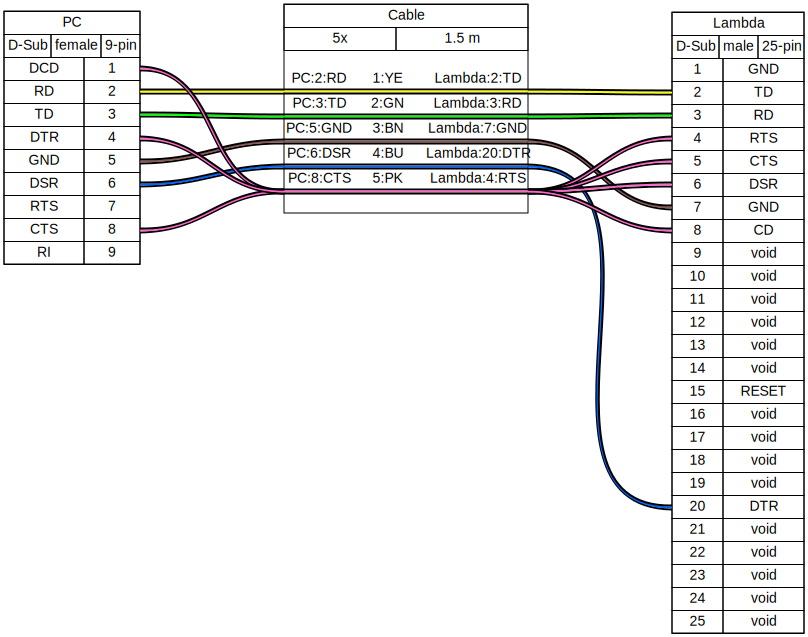
\includegraphics[width=1\textwidth]{cableLambda.png}
	\caption{Shéma de cablage entre l'ordinateur et le Lambda 9}
	\label{fig:cableLambda}
\end{figure}
\end{document}

